\begin{figure}[h]
\centering

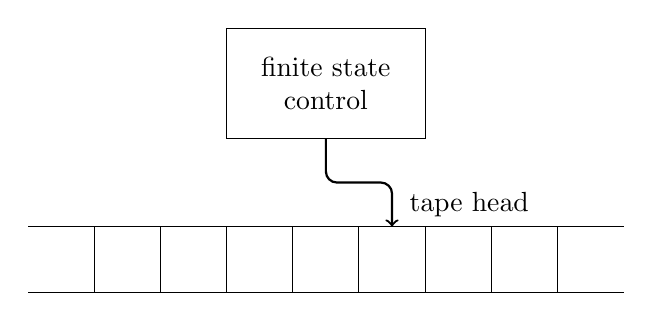
\begin{tikzpicture}[scale=1.4]
    \draw (5.5,1) rectangle (7.3,2);
    
    \node[text width = 2cm, align = center] at (6.4,1.5) {finite state control};

    \draw[thick] [->] {[rounded corners] (6.4,1) -- (6.4,0.6) -- (7,0.6) -- (7,0.2)};

    \node at (7.7,0.4) {tape head};

	\draw (3.7,0.2) -- (4.3,0.2) -- (4.3,-0.4) -- (3.7,-0.4);
	\draw (4.3,0.2) rectangle (4.9,-0.4);
	\draw (4.9,0.2) rectangle (5.5,-0.4);
	\draw (5.5,0.2) rectangle (6.1,-0.4);
	\draw (6.1,0.2) rectangle (6.7,-0.4);
	\draw (6.7,0.2) rectangle (7.3,-0.4);
	\draw (7.3,0.2) rectangle (7.9,-0.4);
	\draw (7.9,0.2) rectangle (8.5,-0.4);
	\draw (9.1,-0.4) -- (8.5,-0.4) -- (8.5,0.2) -- (9.1,0.2);

\end{tikzpicture}


\begin{tikzpicture}[scale=1.4]
	
	\node at (4.6,0.9) {-3};
	\node at (5.2,0.9) {-2};
	\node at (5.8,0.9) {-1};
	\node at (6.4,0.9) {0};
	\node at (7.0,0.9) {1};
	\node at (7.6,0.9) {2};
	\node at (8.2,0.9) {3};

\end{tikzpicture}

\caption{A one-tape DTM that has been initialised.}
\label{fig:DTMModel}
\end{figure}